\begin{tcolorbox}[title=TODO]
Developed architecture / system design / implementation: 1/3

\begin{itemize}
\item start with a theoretical approach
\item describe the developed system/algorithm/method from a high-level point of view
\item go ahead in presenting your developments in more detail
\end{itemize}
\end{tcolorbox}

\section{Approach}
\subsection{Creating Nix Packages}
\begin{tcolorbox}[title=TODO]
\begin{itemize}
    \item Describe why Azure IoT software has to be packaged,
    \item Describe the process of creating Nix packages,
    \item Highlight some key findings.
\end{itemize}
\end{tcolorbox}

\subsection{Conducting Experiments}
\section{Testing Environment}
\subsection{Software}
\subsection{Target Hardware}
\subsection{Build Host}
During the experiments conducted in this thesis, it was required to compile,
package, and build various software. Creating the \ac{OS} variants required a
computationally expensive
creation of an installable image. For building the
various \ac{OS}s and software packages the following hardware was used:

\begin{itemize}
    \item Processor: AMD Ryzen 7 5700X,
    \item Memory: 32 GB (Additionally 64 GB swapped),
    \item Storage: 512 GB SSD.
\end{itemize}

\noindent
A test build was performed with a significantly less powerful machine than the
one presented here, which were not able to complete the build.
Further, the following software versions were used on the build host:
\begin{itemize}
    \item Linux 6.5.6,
    \item Git 2.42.0,
    \item Nix 2.18.1,
    \item GCC 13.2.1 20230801,
    \item Make 4.4.1.
\end{itemize}

\section{Experiments}

\subsection{Base Image Size}

\clearpage
\subsection{Update Image size}
\label{sec:update-image}
When updating the operating system with an A/B failover model, the entire
image needs to be downloaded and written to a secondary partition. In this
\ac{OTA} scenario the size of the operating system image is critical.
For this experiment two sizes are relevant, when comparing operating systems.
Firstly, the actual size of the image that needs to be written to the partition.
Secondly, the size that the entire system takes up on the disk after booting.

\clearpage
\subsection{Time To Recover}
Customers of certain industries require high availability and reliability for
their \ac{IIoT} devices and applications. These availability requirements
are commonly legally and formally negotiated in an \ac{SLA} between
the customer and a service provider \cite{msdoc-slas}. An important consideration
for service providers to achieve high availability is the boot time of the
\ac{OS}. However, for this experiment the time to recover is considered,
instead of the actual boot time of the \ac{OS}. For this experiment, we define the
time to recover as the time until Azure IoT Edge runtime is operable again after
an unexpected reboot.

We argue that the time until operability is more relevant for service providers
when defining \ac{SLO}, since the boot process contains serveral steps that are
outside of the scope of the \ac{OS}, for example, hardware, BIOS or the boot
loader \cite{almesberg}.

\subsubsection{Setup}
For this experiment, an outage of the service will be simulated by sending a
\textit{reboot} system call to the kernel with the \code{reboot}
command line tool. Additionally we will use the \code{-f} (\textit{force}) option to
instruct the command line tool to not call the \textit{shutdown} system call,
which results in a faster shutdown of the system \cite{man-reboot}\cite{man-shutdown}.
In order to execute the command, a \ac{SSH} connection to the target machine
needs to be established.

\begin{figure}[H]
    \centering
    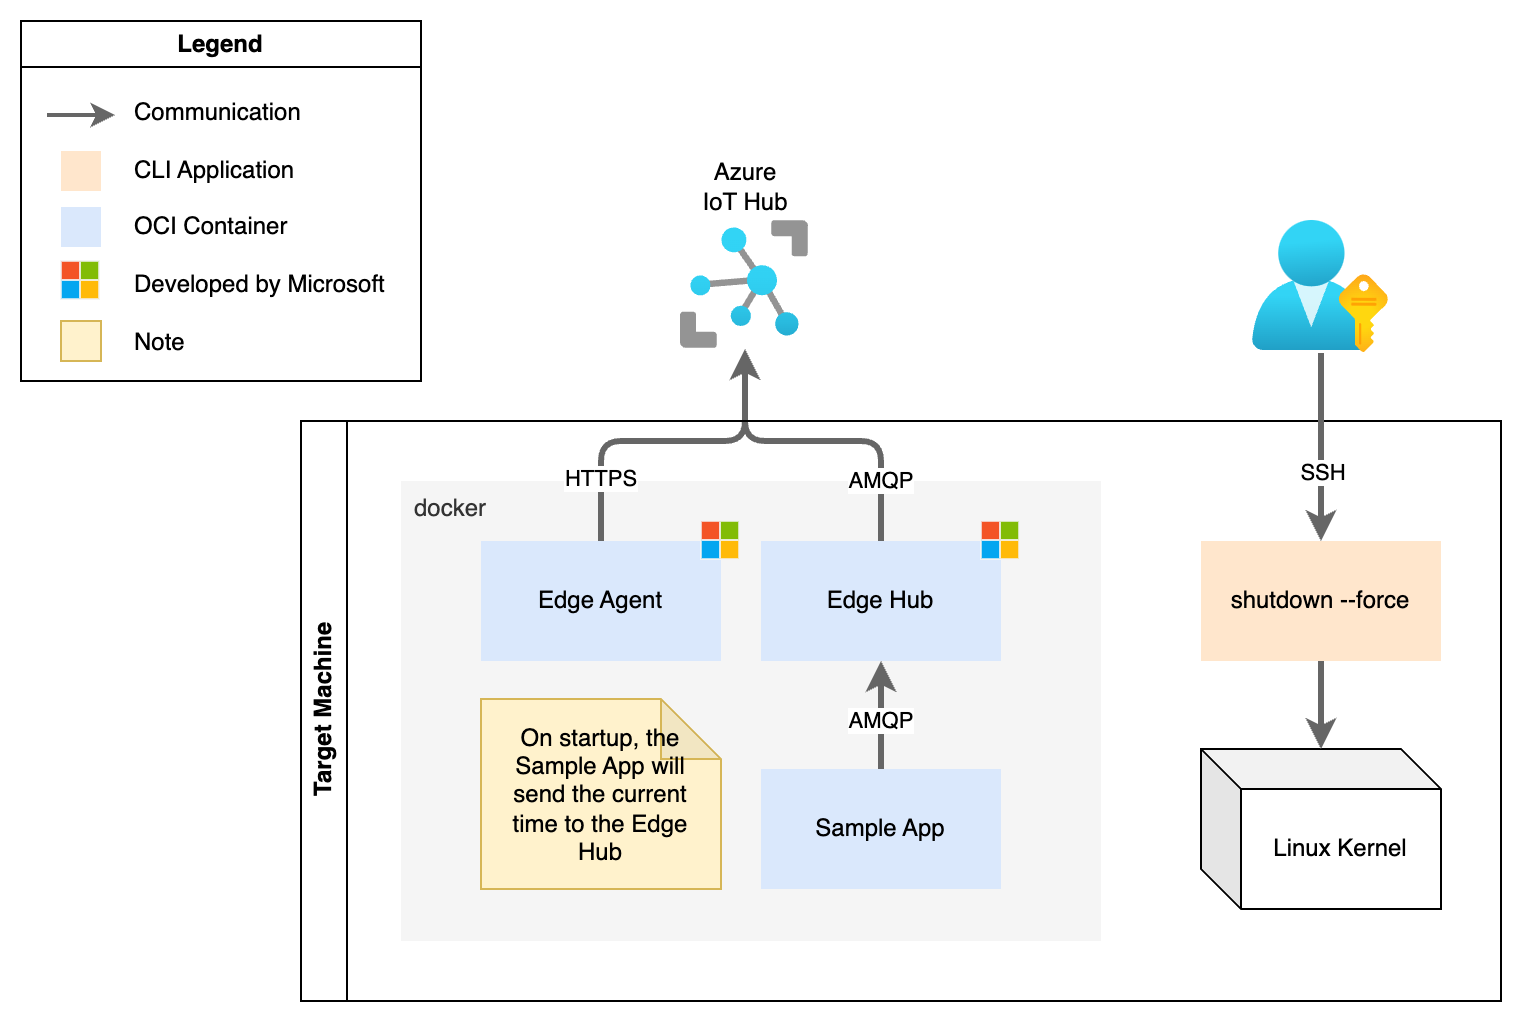
\includegraphics[width=0.75\textwidth]{fig/reboot-setup.drawio.png}
    \caption{Time To Recover Experiment Overview}
\end{figure}

\noindent
Just before the system is rebooted, the current time will be printed.
After the \ac{OS} rebooted and the Azure IoT Edge runtime has started, a
Sample App will send the current time to the Azure IoT Hub via the Azure IoT Edge
Hub, where it can be retrieved. The full shell command can be seen in listing
\ref{lst:reboot-command}.
\\

\begin{lstlisting}[
    caption=Command to print the current time and reboot,
    label=lst:reboot-command]
date +%s \
&& reboot -f
\end{lstlisting}

\noindent
When comparing the first timestamp ($t_0$) from the shell command output with the second
timestamp ($t_1$) from the \textit{Azure IoT Hub}, the time to recover can be calculated,
as the delta between those two timestamps:

\begin{equation}
    T := |t_1 - t_0|
\end{equation}
However, since rebooting the \ac{OS} is a process with many variances, the experiment
must be repeated multiple times. If we repeat the experiment $n$ times, where
$T_i$ represents the result of the $i$-th repetition, we can calculate
a mean value for $T$ as:

\begin{equation}
    \mu := \frac{\sum_{i=1}^{n}T_i}{n}
\end{equation}

\noindent
And the standard deviation for $T$ as:

\begin{equation}
   \sigma := \sqrt{\frac{\sum_{i=1}^{n}((T_i - \mu)^2}{n}}
\end{equation}

\noindent
Finally, the standard error for $T$ as:

\begin{equation}
    s := \frac{\sigma}{\sqrt{n}}
\end{equation}

\noindent
This experiment must be repeated, until the standard error is low enough
to have a confident mean value for each \ac{OS}.

\subsubsection{Hypothesis}
Our hypothesis is, that the time to recover will be very similar for all
\ac{OS}s, since the they all run \textit{Linux}, the Azure IoT Edge runtime and
a similar set of software, such as \textit{systemd} and \ac{SSH}. However, due
to the reduced size of \textit{reUpNix}, we may see a slight advantage in the
time to recover, since the \ac{OS} has to load less data from the disk. Further,
\textit{reUpNix} has a minified kernel and a reduced set of kernel modules.

\clearpage
\subsection{Container Updates}
When using Azure IoT Edge, \ac{IIoT} applications are deployed as containers, because
they change more frequent than the entire \ac{OS}. When a module is updated
with a new deployment manifest, Azure IoT Edge retrieves the any new container
images that are not present on the device. It uses a \ac{UDS} to communicate
with the container runtime, to pull the image. The same can be manually achieved
with the \code{docker pull} command, when using Docker as the container runtime.

\subsubsection{Setup}
\begin{enumerate}
    \item Obtain the container image (e.g. via \code{docker pull} or \code{docker build}),
    \item Fully unpack the image, including all layers,
    \item Merge all layers,
    \item Store the unpacked image in the Nix store,
    \item Include the Nix store object in to the system configuration,
    \item Load the image on boot.
\end{enumerate}
\subsubsection{Hypothesis}
Our hypothesis is, that updating containers with \textit{reUpNix}'s differential
update mechanism will be more efficient than updating them with Azure IoT Edge or
the \code{docker pull} command. This is due to the fact that, if the uppermost
layer of a container image, only contains minimal changes (e.g. only a few
changed files), the differential update will only transmit the changed files in
that layer, instead of the entire layer.
